\documentclass[aspectratio=169,11pt]{beamer}
\usepackage[T1]{fontenc}
\usepackage{booktabs}
\usepackage{graphicx}
\graphicspath{{./}{slides/}}
\renewcommand{\familydefault}{\sfdefault}
\definecolor{accent}{HTML}{1F2A44}
\definecolor{ink}{HTML}{222222}
\setbeamercolor{normal text}{fg=ink,bg=white}
\setbeamercolor{frametitle}{fg=accent,bg=white}
\setbeamercolor{title}{fg=accent,bg=white}
\setbeamercolor{itemize item}{fg=accent}
\setbeamerfont{frametitle}{series=\bfseries,size=\Large}
\setbeamertemplate{navigation symbols}{}
\setbeamertemplate{headline}{}
\setbeamertemplate{itemize item}{--}
\setbeamertemplate{footline}{\hfill\insertframenumber\hspace{1em}\vspace{0.8em}}
\title{Pretrained Models for BirdCLEF+ 2025: Accuracy and CPU Inference Speed}
\subtitle{SC4000 late submissions, Member 3}
\author{Author One, Author Two, Author Three, Author Four}
\institute{Nanyang Technological University}
\date{}
\begin{document}
\begin{frame}[plain]
\titlepage
\end{frame}
\addtocounter{framenumber}{-1}

\begin{frame}{Problem and constraints}
\begin{itemize}
\item 206 classes, about 700 test soundscapes, 12 windows each
\item Metric: macro ROC-AUC
\item Train on focal clips, test on field soundscapes
\item CPU only, no internet, 90 min (our budget: 75)
\item Late submissions, not ranked
\end{itemize}
\note{BirdCLEF+ 2025 asks for the species present in every five-second window of one-minute soundscapes from Colombia. There are 206 classes: birds, amphibians, insects and mammals, scored by macro ROC-AUC. Training data are mostly clean single-species recordings, but the test data are noisy field recordings, so models must transfer between domains. The submission notebook runs on CPU only, without internet, for at most 90 minutes. We set our own budget of 75 minutes. We used late submissions, which do not count for ranking. Next, the baseline we started from.}
\end{frame}

\begin{frame}{Baseline v2 and research question}
\begin{itemize}
\item v2: EfficientNet-B0, ImageNet weights, log-mel input
\item Public 0.763, private 0.789
\item Cut-off 0.776 public; team goal 0.810
\item Question: change only the pretrained model
\item What is the gain, and what is the CPU cost?
\end{itemize}
\note{Our starting point is baseline v2, from a teammate. It is an EfficientNet-B0 with ImageNet weights, reading log-mel spectrograms. It scored 0.763 public and 0.789 private. The grading cut-off is 0.776 on the public split, and the team goal is 0.810. Our question is narrow. If we keep the training recipe, the split and the inference protocol fixed, and change only the pretrained model, how much does the score improve, and what does it cost in CPU time? That sets up the three model families.}
\end{frame}

\begin{frame}{Three pretrained families}
\begin{itemize}
\item \textbf{A1}: bird-pretrained EfficientNetV2-S backbone, v2 head
\item \textbf{A2}: frozen Perch 2.0 (1536-d) + MLP
\item \textbf{A3}: frozen Bird-MAE-Base (768-d) + MLP
\item Perch 2.0 appeared after BirdCLEF 2025 closed: no comparison with official ranks
\end{itemize}
\note{We tried three families. A1 replaces the backbone with a bird-pretrained EfficientNetV2-S from the second-place team. This is a backbone change, not a weights-only swap, and we kept v2's head. A2 uses frozen Perch 2.0 embeddings, 1536 numbers per window, with a small MLP head. A3 uses frozen Bird-MAE-Base features, 768 numbers per window, also with an MLP head. Perch 2.0 was released after the competition closed, so A2 is not comparable to official ranks. Next, how we compared them.}
\end{frame}

\begin{frame}{Experimental protocol}
\begin{itemize}
\item v2 recipe and split fixed (stratified 80/20, seed 42)
\item One seed, one submission per model
\item Public gaps below 0.01 treated as noise
\item 20-file dry run; submit only if projected $\le$ 75 min
\item No labelled soundscapes: validation is focal clips only
\end{itemize}
\note{Every experiment used v2's split: stratified 80/20, seed 42. Each configuration was trained once, with one seed, and submitted once. We treat public differences under 0.01 as noise. Before submitting, a 20-file dry run on unlabelled soundscapes projected the runtime for 700 files, and we submitted only if the projection was at most 75 minutes. There are no labelled soundscapes, so validation uses focal clips only. Validation AUC scores the first five seconds of each clip. Now the results.}
\end{frame}

\begin{frame}{Results}
\small
\begin{tabular}{lrrrrl}
\toprule
Experiment & Val AUC & Public & Private & $\Delta$ public & CPU min / 700 files \\
\midrule
v2 baseline & n/r & 0.763 & 0.789 & 0 & 11.1 measured \\
A1 V2-S bird-pretrained & 0.9832 & 0.82822 & 0.81642 & +0.065 & $\sim$37 projected \\
A2 Perch 2.0 + MLP & 0.9916 & \textbf{0.84774} & \textbf{0.85226} & +0.085 & 25.0 projected \\
A3 Bird-MAE-Base + MLP & 0.9749 & 0.77640 & 0.78016 & +0.013 & 61.6 projected \\
\bottomrule
\end{tabular}

\vspace{1.2em}
{\footnotesize Val AUC: first 5 s of held-out focal clips; n/r = not recorded. Cut-off 0.776 public; team goal 0.810. One seed, one submission each.}
\note{Here are the leaderboard results. A2, Perch with an MLP, is best: 0.84774 public and 0.85226 private. A1 follows with 0.82822 and 0.81642. Both clear the team goal of 0.810 on both splits. A3 scores 0.77640 and 0.78016, which is no reliable gain. Validation AUC was high for all three and understated the gaps, so we choose by leaderboard. A2's validation may be inflated by overlap with Perch's training data. The CPU times for A1, A2 and A3 are projections. Next, a bias finding.}
\end{frame}

\begin{frame}{Bias initialisation finding}
\small
\begin{tabular}{llc}
\toprule
Features and head & Bias init & First-5s val AUC \\
\midrule
Bird-MAE, linear & default & 0.7498 \\
Bird-MAE, linear & log-prior & 0.9626 \\
Bird-MAE, MLP (submitted) & default & 0.9749 \\
Bird-MAE, MLP & log-prior & 0.9707 \\
\bottomrule
\end{tabular}

\vspace{1.2em}
\begin{itemize}
\item Cause is likely, not proven; validation only
\item Perch logistic regression (0.9071): presumed same defect, not rerun
\end{itemize}
\note{One finding is practical. A linear probe on Bird-MAE features scored 0.7498 with default bias initialisation, and 0.9626 with the bias set to the class log-prior. The cause is likely that a bias starting near zero cannot reach about minus six under a low learning rate. That distance is an analytical estimate, not a measurement. For the MLP, the log-prior did not help: 0.9707 against 0.9749. The Perch logistic regression probably has the same defect, but we did not rerun it. Now, why A3 did not help.}
\end{frame}

\begin{frame}{Reading A3}
\begin{itemize}
\item Public 0.77640: above the cut-off by 0.0004 (noise)
\item Private 0.78016: 0.009 below v2
\item No claim of improvement
\item Hypotheses, untested: mean pooling loses patch structure; overlapping species in one window; features encode background
\item Prototypical probe not run
\end{itemize}
\note{A3 gives no clear gain. Its public score of 0.77640 clears the 0.776 cut-off by only 0.0004, which is noise. Its private score is 0.009 below v2, and the two splits disagree in sign. We make no claim that it improved. We have three hypotheses, none tested. First, mean pooling discards the structure of the patch map. Second, one pooled vector may represent overlapping species poorly. Third, self-supervised features may encode background as strongly as call identity. We did not run a prototypical probe. Next, inference speed.}
\end{frame}

\begin{frame}{Inference speed}
\begin{itemize}
\item Whole notebook: v2 11.1 $\to$ 5.5 min; A1 8.0 min
\item Pipeline only: v2 10.4 $\to$ 4.0 min; A1 7.2 min
\item Measured on 700 files; changes bundled, not attributed
\end{itemize}
\begin{center}
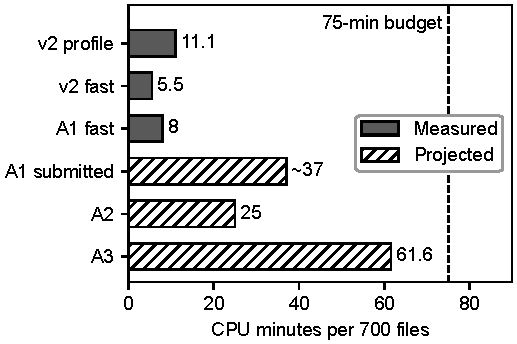
\includegraphics[height=0.46\textheight]{figures/timing_chart.pdf}
\end{center}
\note{For speed, the fast pipeline uses four workers with one thread each, one mel call per file, and batched windows. Compared like with like, the whole notebook for v2 fell from 11.1 to 5.5 minutes, and A1 takes 8.0. For the pipeline alone, v2 fell from 10.4 to 4.0 minutes, and A1 takes 7.2. These are measured on 700 soundscapes. The changes were bundled, so we cannot attribute the speedup. The submitted notebooks did not use this pipeline, so their times are projections. Last, limitations and conclusions.}
\end{frame}

\begin{frame}{Limitations, next steps, conclusion}
\begin{itemize}
\item Limits: single seed, no labelled soundscapes, A2 validation possibly inflated, A1 confounded
\item Next: noisy-student loop, prototypical probe, ImageNet control for A1
\item A1 and A2 raised public 0.763 to 0.828 and 0.848
\item A3: no reliable gain
\item A1--A3 CPU times are projections
\end{itemize}
\note{Limitations: one seed, noisy public scores, no labelled soundscapes, and possible validation inflation for A2. A1 also confounds architecture, pretraining and normalisation. Next steps are a noisy-student loop with a strong teacher, a prototypical probe for Bird-MAE, and an ImageNet control for A1. In conclusion, changing only the pretrained model raised the public score from 0.763 to 0.82822 with A1 and 0.84774 with A2. A3 gave no reliable gain. Local validation understated the gaps, and the CPU times for A1 to A3 are projections.}
\end{frame}
\end{document}
